\usetikzlibrary{arrows.meta,automata,positioning,shadows}
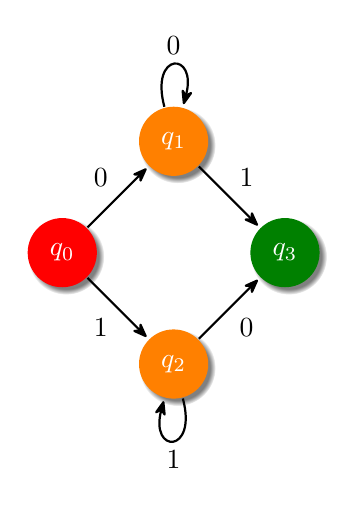
\begin{tikzpicture}[shorten >=1pt,node distance=2cm,on grid,
  >={Stealth[round]},thick,
  every state/.style={fill,draw=none,orange,text=white,circular drop shadow},
  accepting/.style={green!50!black,text=white},
  initial/.style={red,text=white}]
\node[state,initial] (q_0) {$q_0$};
\node[state] (q_1) [above right=of q_0] {$q_1$};
\node[state] (q_2) [below right=of q_0] {$q_2$};
\node[state,accepting](q_3) [below right=of q_1] {$q_3$};
\path[->] (q_0) edge node [above left] {0} (q_1)
   edge node [below left] {1} (q_2)
   (q_1) edge node [above right] {1} (q_3)
   edge [loop above] node {0} ()
   (q_2) edge node [below right] {0} (q_3)
   edge [loop below] node {1} ();
\end{tikzpicture}
